% Related work

Prior research has already examined the capacity of various machine-learning and data-engineering techniques to classify toxic comments. 
Of general interest to this paper is the literature on sentiment analysis, which combines natural-language-processing (NLP) techniques and opinion mining to emulate human-level comprehension of positive or negative sentiment expressed in textual statements \cite{chowdhary2020natural, cambria2014jumping}.
A relatively new branch of NLP literature considers applications of sentiment-analysis to the task of toxic behaviour. 
Research in this domain can be stratified with respect to the specific dimension of toxic behaviour of interest: besides general classification of toxic online comments \cite{georgakopoulos2018convolutional,van2018challenges,risch2020toxic}, related literature also considers classification of specific dimensions of toxic behaviour, inluding hate speech \cite{mullah2021advances, ayo2020machine, rizos2019augment, yang2019exploring}; harrassessment \cite{abarna2022identification, basu2021cyberpolice, marwa2018deep}; abusive-language \cite{vidgen2020directions, nobata2016abusive, bourgonje2017automatic}; and cyber-bullying \cite{kanan2020cyber, akhter2019cyber, di2016unsupervised}.

With respect to the selection of machine-learning frameworks employed for toxic comment classification, prior research is generally consistent in its advocation of certain machine learning techniques as better-suited for the task of toxic comment classifications. In particular, approaches towards classification of toxicity appear to prefer employment of convolutional neural networks (CNNs) \cite{androcec2020machine}, as these methods are known to excel at tasks involving elements of pattern-recognition. While CNNs are perhaps most well-known for applications in image-recognition \cite{rawat2017deep}, effective translation to sentiment-analysis tasks is unsurprising given the role of syntactical pattern recognition in language comprehension. For example, syntactical patterns such as word order, indiciative pharases, and idioms all modify meaning in a way that is algorithmic and theoretically 'learnable'. Indeed, understanding the implications of such patterns is essential to accurate comprehension of language. 

At the data pre-processing level, a number of studies consider potential for improved toxic-comment classification through pre-processing using  word-embedding techniques, such as TF-IDF \cite{luhn1957statistical, jones1972statistical}, GloVe \cite{pennington2014glove}, Word2Vec \cite{mikolov2013efficient,mikolov2013distributed}, and FastText \cite{bojanowski2017enriching, joulin2016bag, joulin2016fasttext} (for a recent review of these techniques, see Birunda and Devi, 2021 \cite{selva2021review}). These techniques systematically estimate vector representations for words in a specified vocabulary, such that words arising from common contexts exhibit similar vector representations.


% \begin{figure}
% 	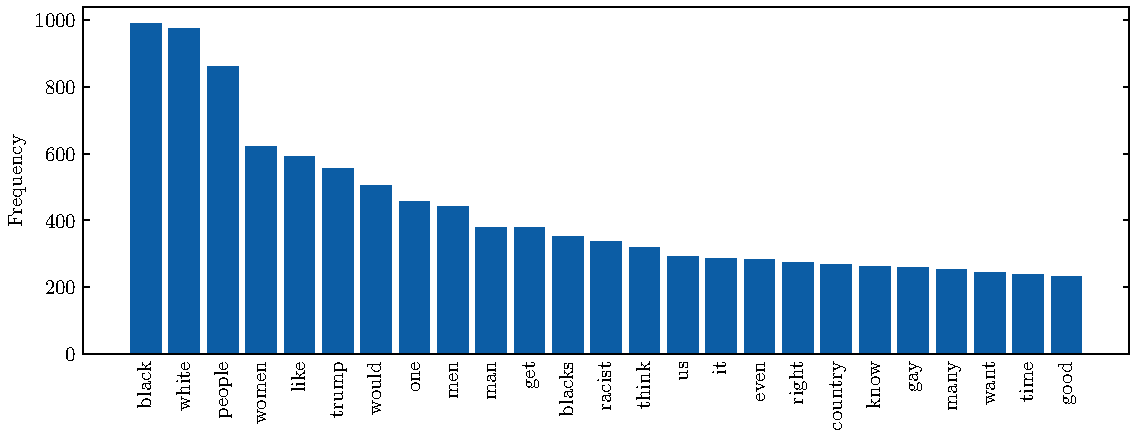
\includegraphics[width=1.0\textwidth]{graphics/toxic_word_freq.pdf}
%     \caption{Words appearing most frequently in toxic comments}
% \end{figure}


% \begin{figure}
% 	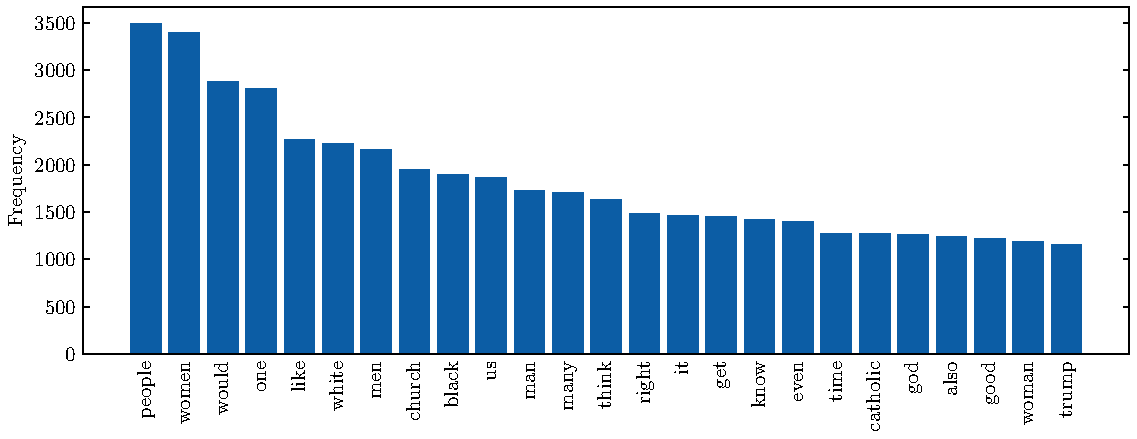
\includegraphics[width=1.0\textwidth]{graphics/nontoxic_word_freq.pdf}
%     \caption{Words appearing most frequently in non-toxic comments}
% \end{figure}